\section{Design Methodology}\label{sec:design}
%% methodology behind how we decided to tackle hill climb and obstacle avoidance
% flowchart here?
\vspace{-0.2cm} Exploring the complexity introduced by an unknown obstacle course led us to abstract key system features via variables and layers and hence designing an Hierarchical Extended Finite State Machine (HFSM). Navigating the obstacle course using a HFSM allows flexibility in control and a level of autonomous decision making by the robot in response to sensor and actuator signals. The two main design challenges of obstacle avoidance and hill climbing were approached separately to simplify the design process. Simulation of the algorithms were used to fine tune the design via CyberSim. The play/pause states were adopted from the templates provided and were tested for feasibility. Overall it was an iterative process going between analysis/design, simulation and deloying/testing. Figure \ref{fig:workflow} depicts the workflow adopted in the design process. The details of implementation, simulation and how we used the Kobuki for testing will be discussed in Section \ref{sec:testing}.
\begin{figure}[H]
    \centering
    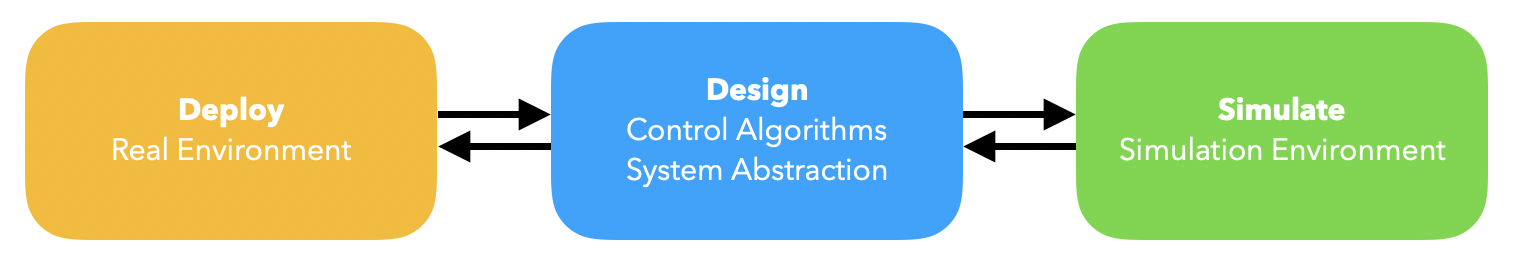
\includegraphics[width=16cm]{Images/Workflow.png}
    \caption{Design workflow \cite[p.~36]{labguide}}
    \label{fig:workflow}
\end{figure}

\clearpage
\subsection{Obstacle Avoidance}\label{sec:obstacle_alg}
\vspace{-0.2cm} The obstacle avoidance algorithm was designed gradually through iteration. Each development cycle introduced new use cases and targeted problems from the previous round. %%% figures of basic FSM required here?
\begin{enumerate}
    \item A minimum viable product (MVP) version of a state machine used for obstacle avoidance was implemented. When the Kobuki collided with an object it would reverse, rotate $90^\circ$ right, travel parallel to the collision point, rotate back into the original line of travel and continue.\\
    \textbf{Success}: This algorithm proved effective at travelling around a single obstacle.\\
    \textbf{Issues}: The Kobuki only rotates right whilst avoiding the obstacle, which means if the right bumper was triggered it would have to a long way around as shown in Figure \ref{fig:Obstacle1}.
    \item The algorithm was improved by rotating the Kobuki away from the obstacle - in the direction opposite to the bumper sensor that was triggered. If the right bumper was pressed then the Kobuki would avoid by rotating left and vice versa. If the centre bumper was pressed, it remains rotating right.\\
    \textbf{Success}: This algorithm proved to be much more efficient at avoiding obstacles by taking a shorter path responding with respect to each sensor.\\
    \textbf{Issues}: If the Kobuki hit an obstacle during the avoiding state it would reverse, rotate and avoid again as seen in Figure \ref{fig:Obstacle2}. This loses the ground orientation and does not meet design requirements.
    \begin{figure}[H]
    \centering
    \begin{minipage}{0.45\textwidth}
        \centering
        \vspace{0.5cm}
        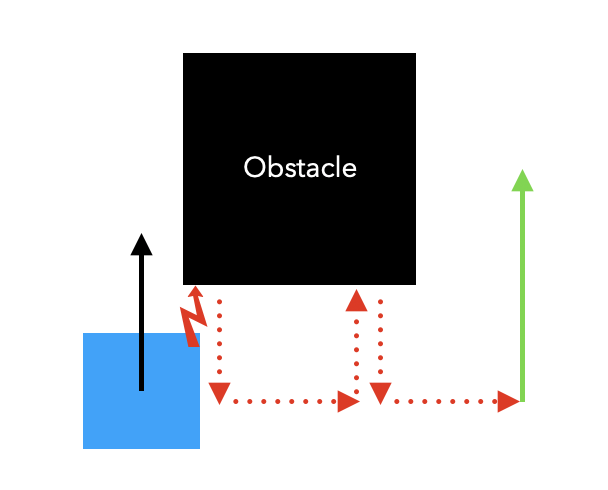
\includegraphics[width=4.6cm]{Images/Obstacle1.png}
        \caption{Inefficient path around an obstacle when the avoidance rotation is solely rotate $90^\circ$ right}
        \label{fig:Obstacle1}
    \end{minipage}%
    \hspace{0.5cm}
    \begin{minipage}{0.45\textwidth}
    \centering
        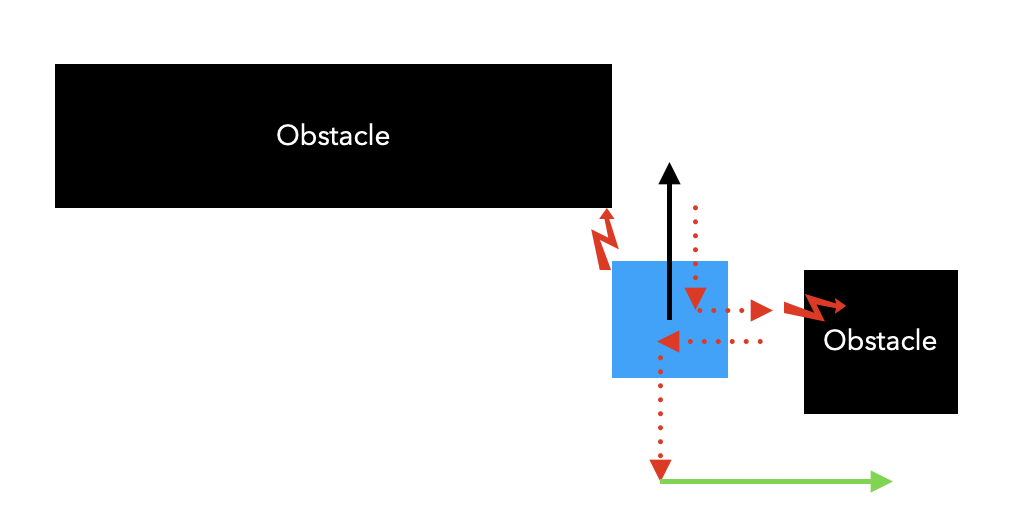
\includegraphics[width=8cm]{Images/Obstacle2.png}
        \caption{Going in the opposite direction to original drive after responding to a second obstacle whilst avoiding the first}
        \label{fig:Obstacle2}
    \end{minipage}
    \end{figure}
    \item The final iteration handled meeting obstacles during the avoiding state. A new state was added to ensure that the Kobuki would rotate back to the ground orientation after the second reverse. Additionally, to avoid getting stuck by rotating back and forth between obstacles, a variable was added to change the direction that the Kobuki turned when the centre bumper was pressed. For example, after the first corner situation the centre bumper would now trigger a left rotate instead of right rotate in avoidance.
    \begin{figure}[H]
        \centering
        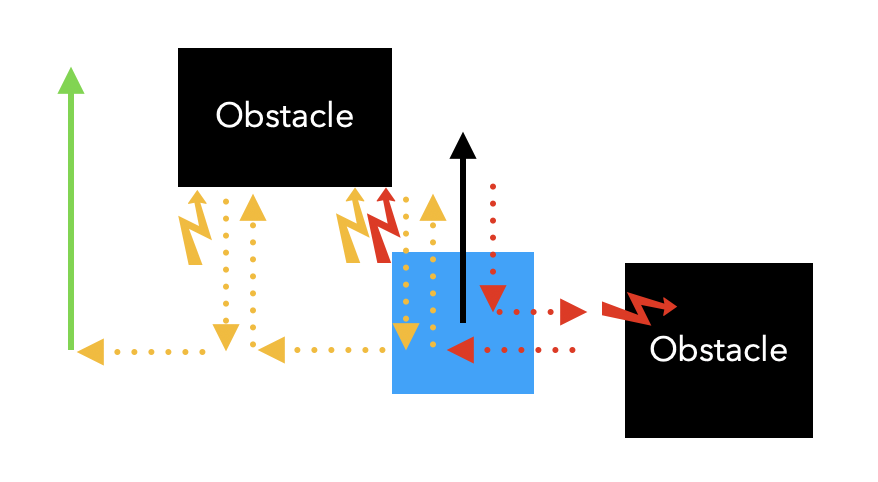
\includegraphics[width=6cm]{Images/Obstacle3.png}
        \caption{Orange arrows show the path after encountering an object whilst in an obstacle avoiding state}
        \label{fig:Obstacle3}
    \end{figure}
\end{enumerate}

\subsection{Hill Climb}\label{sec:hill_alg}
\vspace{-0.2cm} The hill climbing algorithm also went through design iterations for detecting an incline and reorienting to travel directly uphill or downhill. The hill is assumed to slope along one axis only in the obstacle course. However, slope testing in the simulation presented difficulties and are discussed in Section \ref{sec:cybersim}.
\begin{enumerate}
    \item The MVP algorithm used the low pass filtered accelerometer readings in $g$ to detect a hill (see Section \ref{sec:accelerometer_LPF}). An incline was detected when the absolute value of the $z$ accelerometer decreased below a  threshold from $1g$. When on a hill, the Kobuki rotated until the absolute value of the $y$ accelerometer increased beyond a threshold above $0g$.\\
    \textbf{Success}: The algorithm proved responsive to pitch detection for an incline.\\
    \textbf{Issues}: Reorientation was difficult with the accelerometer value from just the $y$ axis as it was too sensitive to fluctuations and wasn't indicating the orientation correctly.
    
    \item Equations in Section \ref{sec:acc} were used to calculate pitch and yaw angles via the accelerometer. Additionally, when the Kobuki is first unpaused $x$, $y$, and $z$ values were set to zero to avoid calibration bias.\\
    \textbf{Success}: Hill detection and hill orientation performance was greatly improved. The reliability of detection improved with the zero initialisation.\\
    \textbf{Issues}: Thresholds set for both pitch and yaw angles for hill orientation showed significant chattering.
    
    \item The final iteration radically changed the way the Kobuki reoriented on a hill. Instead of stopping and rotating until a threshold is met, a feedback loop was introduced. The relative speeds of each wheel were adjusted to be proportional to the difference between the current orientation and the desired orientation. This is shown in Figure \ref{fig:hillARC} in comparison with the chattering path.
    \begin{figure}[H]
        \centering
        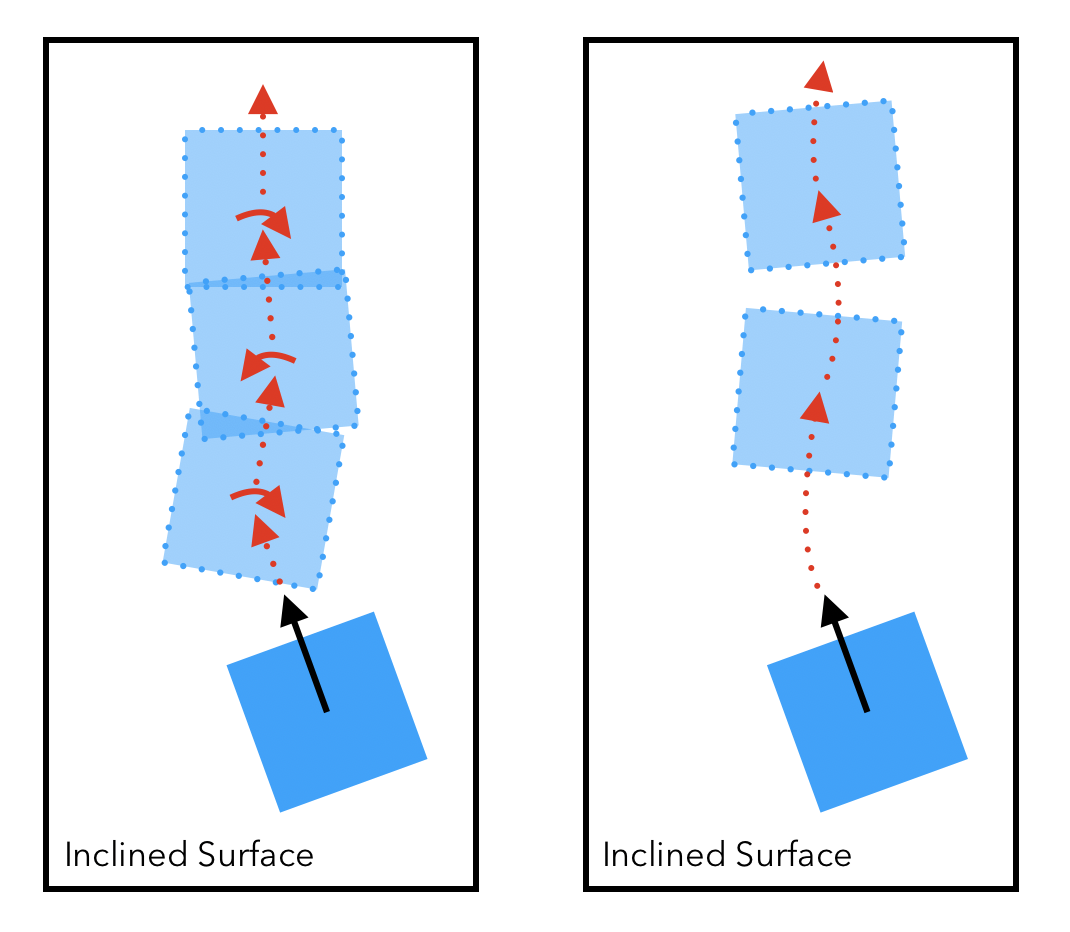
\includegraphics[width=6cm]{Images/ChatterVSArc.png}
        \vspace{-0.2cm}
        \caption{Left: Reorienting path with chattering; Right: Reorienting path with rotation angle feedback}
        \label{fig:hillARC}
    \end{figure}
\end{enumerate}

\subsection{Hierarchical Extended Finite State Machine}\label{sec:FSM}
%A complete FSM diagram (including pause states) of the robot algorithm using the notation covered in the lectures. If you use an Extended state machine, or state refinements, you must show all states, variables and transitions.
\vspace{-0.2cm} There are 3 levels to the final hierarchical extended finite state machine. The run/pause level, the obstacle avoidance level and the hill climbing level. When the system is in the run state, the system enters the state refinement for obstacle avoidance. During the drive state of the obstacle avoidance refinement the system enters another state refinement to handle hill climbing. Note that the transitions to the states with refinements are history transitions - the refinements remember which state they are in rather than resetting. This is crucial for the pause behaviour and for tracking the hill states. This design neatly abstracts the different tasks that the Kobuki must perform. There is also the added benefit of being able to avoid obstacles while hill climbing - no additional states are required to avoid cliffs. The state diagram is shown in Figure \ref{fig:FSM}. Trigger and action labels are used to simplify the diagram, see Tables \ref{tab:triggers} and \ref{tab:actions} for the label definitions. The output converter in Table \ref{tab:outputs} uses the variable \textit{DriveMode} to convert to the left and right wheel speeds on each update. The \textit{incline} and \textit{tiltAngle} variables are calculated on each update according to the pitch and yaw calculations of Section \ref{sec:acc}. % consider flowchart?

\begin{figure}[p]
    \centering
    \begin{tabular}{ll}
      \textbf{inputs:}   & \textit{B0} : pure\\
                         & \textit{cliffLeft, cliffCentre, cliffRight} : pure \\
                         & \textit{bumpLeft, bumpCenter, bumpRight} : pure \\
                         & \textit{wheelDropLeft, wheelDropRight} : pure\\
                         & acc : $\mathbb{R}^3$\\
                         & \textit{netAngle, netDistance} : $\mathbb{R}$\\
      \textbf{variables:}& \textit{driveMode} : \{FORWARD, BACKWARD, ROTATE\_LEFT, ROTATE\_RIGHT, ARC, STOP\}\\
                         & \textit{incline, tiltAngle} : $\mathbb{R}$\\
                         & \textit{turnPct} : $\mathbb{R}$\\
                         & \textit{distance, angle} : $\mathbb{R}$\\
                         & \textit{obstacleLoc} : \{LEFT, CENTRE, RIGHT\}\\
                         & \textit{offsets} : $\mathbb{R}^3$\\
                         & \textit{centreTurn} : \{\textit{true, false}\}\\
     \textbf{outputs:}   & \textit{leftWheelSpeed}, \textit{rightWheelSpeed} :  $\mathbb{R}$\\
    \end{tabular}
    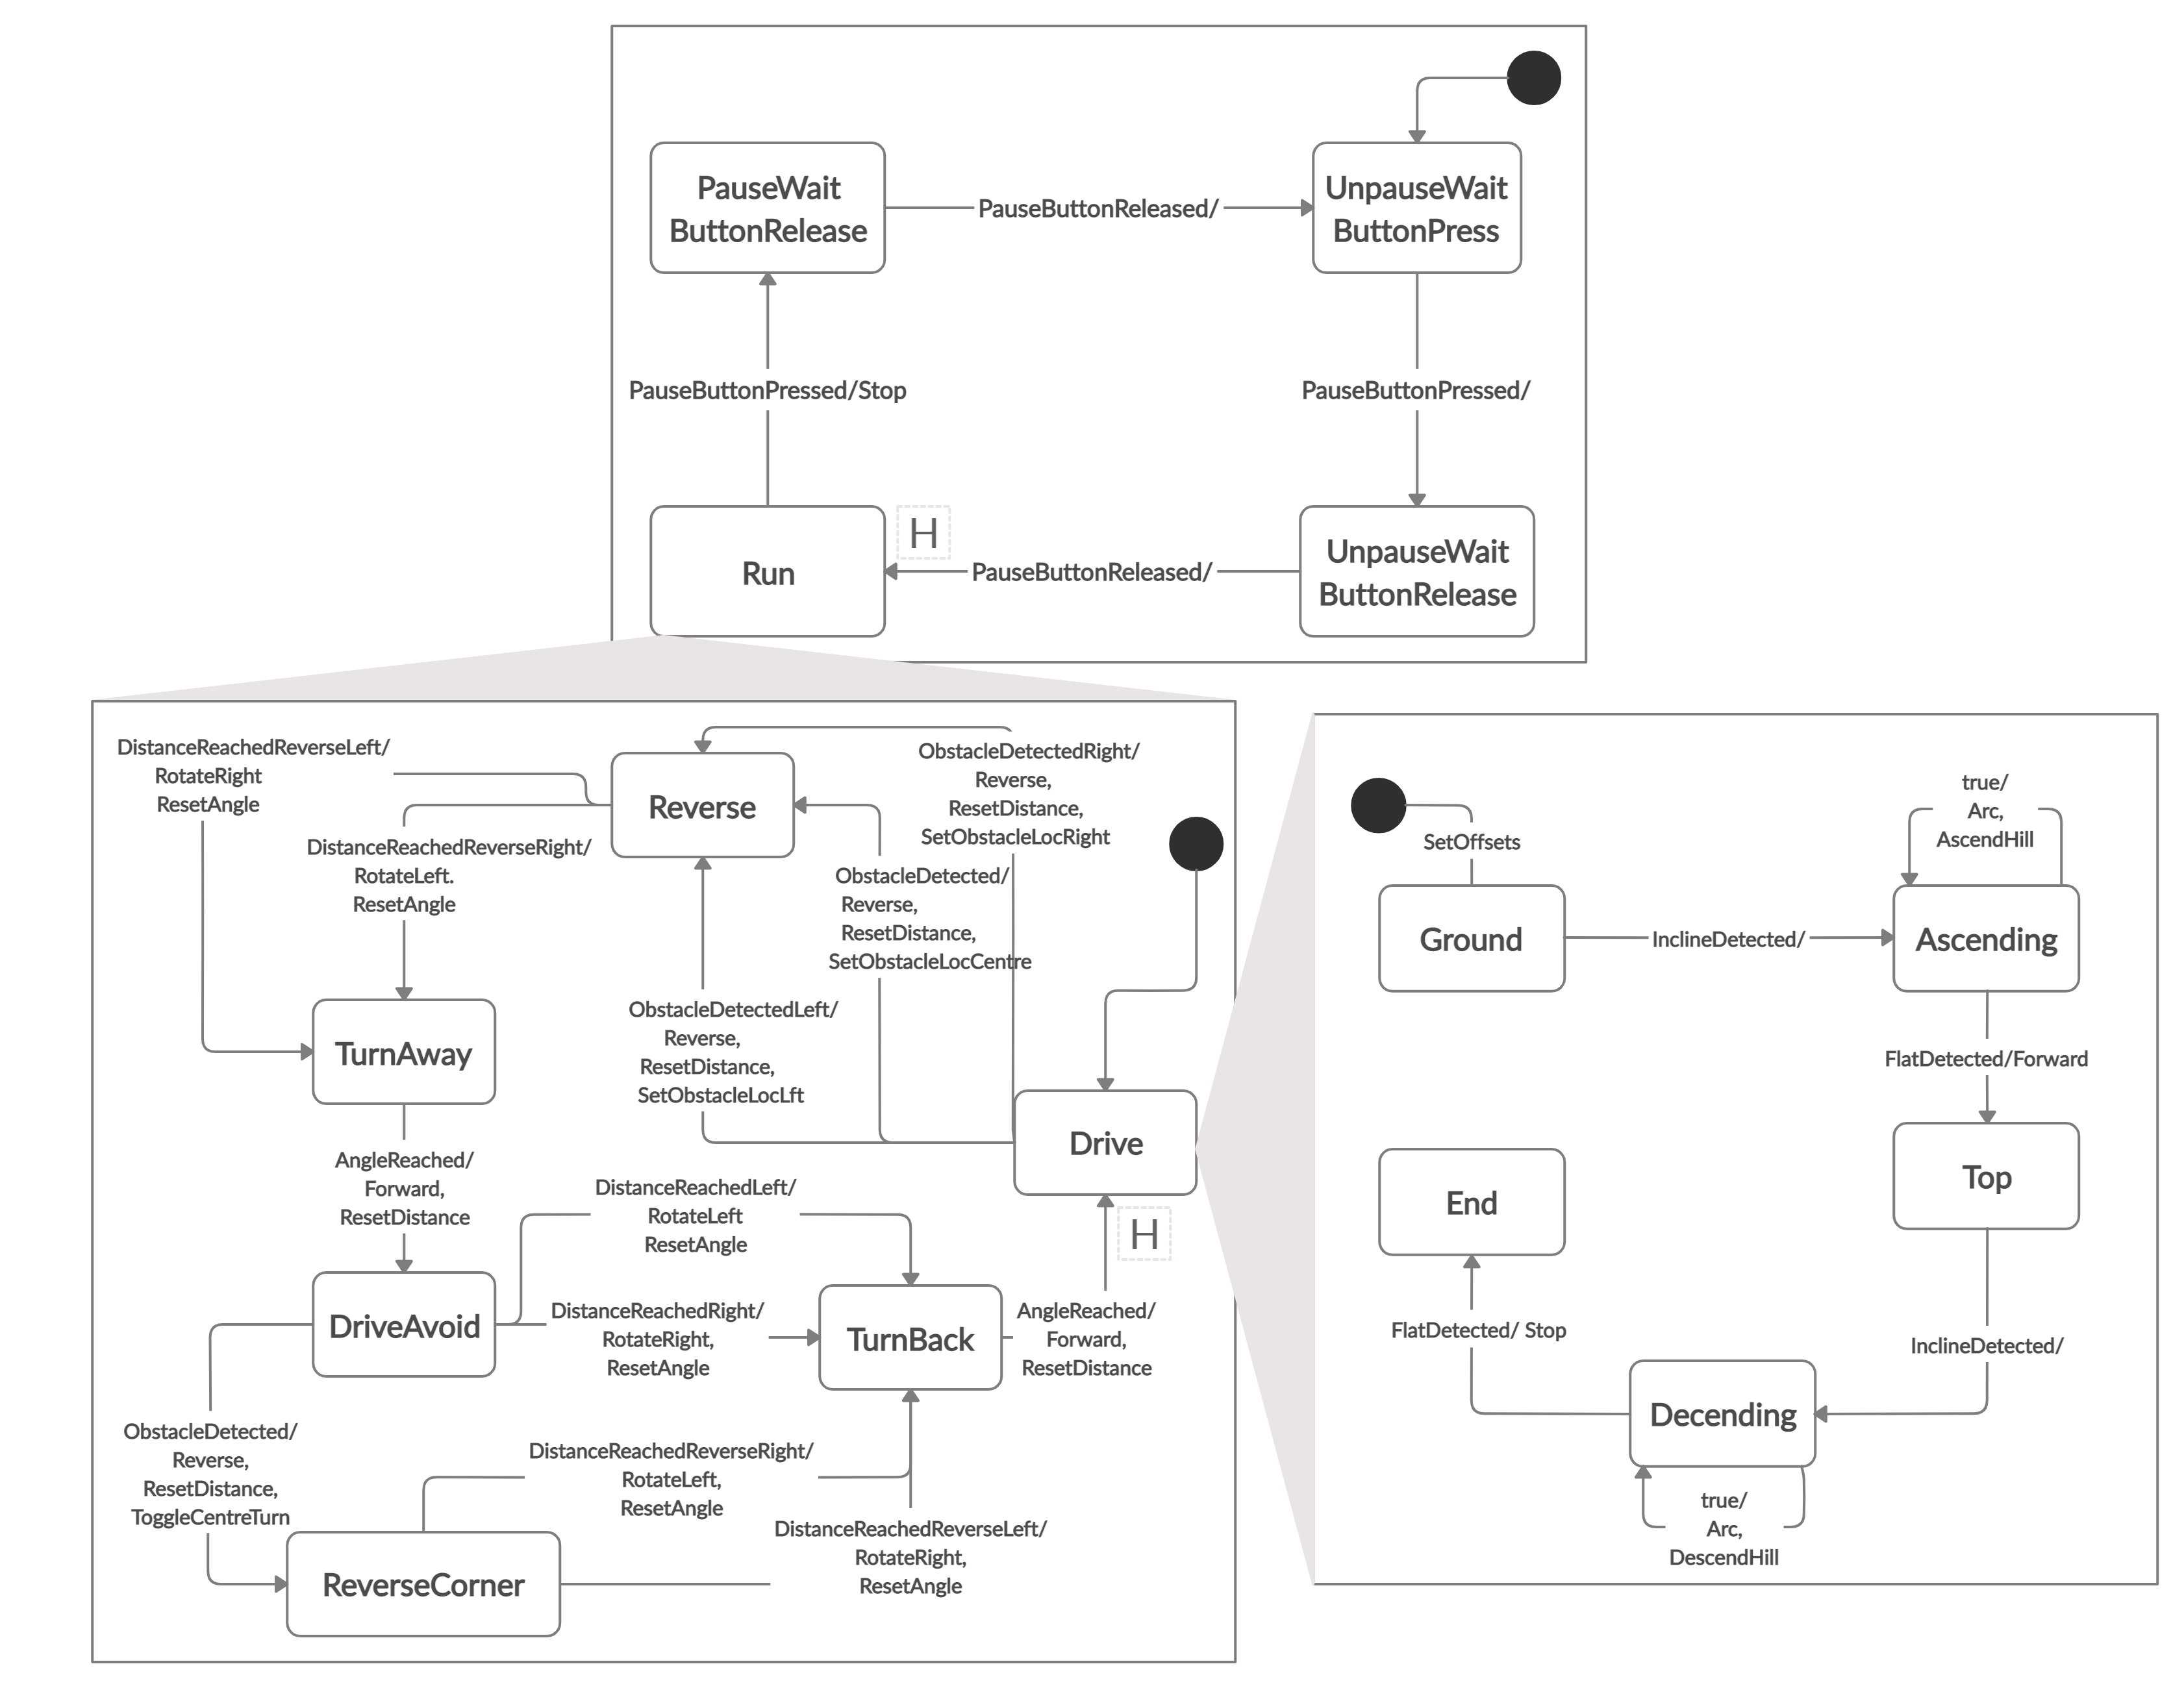
\includegraphics[width=\textwidth]{Images/Finite_State_Machine_v2.png}
    \caption{Extended State Machine (See Tables \ref{tab:triggers} and \ref{tab:actions} for Trigger and Action definitions)}
    \label{fig:FSM}
\end{figure}

\begin{table}[p]
    \centering
    \begin{tabular}{|c|c|}
        \hline
        Name        & Trigger Definition \\
        \hline\hline
        PauseButtonPressed & \textit{B0} \\
        \hline
        PauseButtonReleased    & $\neg$\textit{B0}  \\
        \hline
        ObstacleDetectedLeft & \textit{cliffLeft} $\lor$ \textit{bumpLeft} $\lor$ \textit{wheelDropLeft}\\
        \hline
        ObstacleDetectedRight & \textit{cliffRight} $\lor$ \textit{bumpRight} $\lor$ \textit{wheelDropRight}\\
        \hline
        ObstacleDetectedCentre & \textit{cliffCentre} $\lor$ \textit{bumpCentre}\\
        \hline
        ObstacleDetected & ObstacleDetectedLeft $\lor$ ObstacleDetectedRight $\lor$ ObstacleDetectedCentre\\
        \hline
        DistanceReached & abs(\textit{netDistance} - \textit{distance}) $\geq$ distanceReachedThreshold\\
        \hline
        DistanceReachedLeft & DistanceReached $\land$ (\textit{obstacleLoc} = LEFT $\lor$ \textit{centreTurn})\\
        \hline
        DistanceReachedRight & DistanceReached $\land$ $\neg$(\textit{obstacleLoc} = LEFT $\lor$ \textit{centreTurn})\\
        \hline
        DistanceReachedReverse & abs(\textit{netDistance} - \textit{distance}) $\geq$ distanceReachedReverseThreshold\\
        \hline
        DistanceReachedReverseLeft & DistanceReachedReverse $\land$ (\textit{obstacleLoc} = LEFT $\lor$ \textit{centreTurn})\\
        \hline
        DistanceReachedReverseRight & DistanceReachedReverse $\land$ $\neg$(\textit{obstacleLoc} = LEFT $\lor$ \textit{centreTurn})\\
        \hline
        AngleReached & abs(\textit{netAngle} - \textit{angle}) $\geq$ 90\\
        \hline
        FlatDetected & abs(\textit{incline)} $<$ flatDetectedThreshold\\
        \hline
        InclineDetected & abs(\textit{incline}) $>$ inclineDetectedThreshold\\
        \hline
    \end{tabular}
    \caption{Trigger Definitions}
    \label{tab:triggers}
\end{table}

\begin{table}[p]
    \centering
    \begin{tabular}{|c|c|}
        \hline
        Name        & Action Definition \\
        \hline\hline
        SetObstacleLocLeft & \textit{obstacleLoc} := LEFT \\
        \hline
        SetObstacleLocRight & \textit{obstacleLoc} := RIGHT \\
        \hline
        SetObstacleLocCentre & \textit{obstacleLoc} := CENTRE \\
        \hline
        ResetDistance & \textit{distance} := \textit{netDistance}\\
        \hline
        ResetAngle & \textit{angle} := \textit{netAngle}\\
        \hline
        Forward & \textit{driveMode} := FORWARD \\
        \hline
        Reverse & \textit{driveMode} := BACKWARD \\
        \hline
        RotateRight & \textit{driveMode} := ROTATE\_RIGHT \\
        \hline
        RotateLeft & \textit{driveMode} := ROTATE\_LEFT \\
        \hline
        Stop & \textit{driveMode} := STOP \\
        \hline
        Arc & \textit{driveMode} := ARC \\
        \hline
        AscendHill & \textit{turnPct} := $-\textit{tiltAngle}/\pi$\\
        \hline
        DescendHill & \textit{turnPct} := $-(\textit{tiltAngle}-\text{sign(\textit{tiltAngle})}\pi)/\pi$\\
        \hline
        ToggleCentreTurn & \textit{centreTurn} := $\neg$ \textit{centreTurn}\\
        \hline
        SetOffsets & \textit{offsets}:= \{\textit{acc.x}, \textit{acc.y}, $1.0-\textit{acc.z}$\}\\
        \hline
    \end{tabular}
    \caption{Action Definitions}
    \label{tab:actions}
\end{table}

\begin{table}[p]
    \centering
    \begin{tabular}{|c|c|c|}
        \hline
        \textit{DriveMode}  & \textit{leftWheelSpeed} & \textit{rightWheelSpeed} \\
        \hline\hline
        FORWARD & SPEED & SPEED \\
        \hline
        BACKWARD & $-$SPEED & $-$SPEED \\
        \hline
        ROTATE\_LEFT & $-$SPEED & SPEED \\
        \hline
        ROTATE\_RIGHT & SPEED & $-$SPEED \\
        \hline
        ARC & $\text{SPEED}(1.0-\textit{turnPct})$ & $\text{SPEED}(1.0+\textit{turnPct})$ \\
        \hline
        STOP & 0 & 0\\
        \hline
    \end{tabular}
    \caption{Output Converter}
    \label{tab:outputs}
\end{table}

% I feel like we need to discuss more here?
% describe key states? 
% how many states, efficiency etc... 
% why we decided on hierarchical